% Options for packages loaded elsewhere
\PassOptionsToPackage{unicode}{hyperref}
\PassOptionsToPackage{hyphens}{url}
%
\documentclass[
  ignorenonframetext,
]{beamer}
\usepackage{pgfpages}
\setbeamertemplate{caption}[numbered]
\setbeamertemplate{caption label separator}{: }
\setbeamercolor{caption name}{fg=normal text.fg}
\beamertemplatenavigationsymbolsempty
% Prevent slide breaks in the middle of a paragraph
\widowpenalties 1 10000
\raggedbottom
\setbeamertemplate{part page}{
  \centering
  \begin{beamercolorbox}[sep=16pt,center]{part title}
    \usebeamerfont{part title}\insertpart\par
  \end{beamercolorbox}
}
\setbeamertemplate{section page}{
  \centering
  \begin{beamercolorbox}[sep=12pt,center]{part title}
    \usebeamerfont{section title}\insertsection\par
  \end{beamercolorbox}
}
\setbeamertemplate{subsection page}{
  \centering
  \begin{beamercolorbox}[sep=8pt,center]{part title}
    \usebeamerfont{subsection title}\insertsubsection\par
  \end{beamercolorbox}
}
\AtBeginPart{
  \frame{\partpage}
}
\AtBeginSection{
  \ifbibliography
  \else
    \frame{\sectionpage}
  \fi
}
\AtBeginSubsection{
  \frame{\subsectionpage}
}
\usepackage{amsmath,amssymb}
\usepackage{iftex}
\ifPDFTeX
  \usepackage[T1]{fontenc}
  \usepackage[utf8]{inputenc}
  \usepackage{textcomp} % provide euro and other symbols
\else % if luatex or xetex
  \usepackage{unicode-math} % this also loads fontspec
  \defaultfontfeatures{Scale=MatchLowercase}
  \defaultfontfeatures[\rmfamily]{Ligatures=TeX,Scale=1}
\fi
\usepackage{lmodern}
\ifPDFTeX\else
  % xetex/luatex font selection
\fi
% Use upquote if available, for straight quotes in verbatim environments
\IfFileExists{upquote.sty}{\usepackage{upquote}}{}
\IfFileExists{microtype.sty}{% use microtype if available
  \usepackage[]{microtype}
  \UseMicrotypeSet[protrusion]{basicmath} % disable protrusion for tt fonts
}{}
\makeatletter
\@ifundefined{KOMAClassName}{% if non-KOMA class
  \IfFileExists{parskip.sty}{%
    \usepackage{parskip}
  }{% else
    \setlength{\parindent}{0pt}
    \setlength{\parskip}{6pt plus 2pt minus 1pt}}
}{% if KOMA class
  \KOMAoptions{parskip=half}}
\makeatother
\usepackage{xcolor}
\newif\ifbibliography
\usepackage{graphicx}
\makeatletter
\def\maxwidth{\ifdim\Gin@nat@width>\linewidth\linewidth\else\Gin@nat@width\fi}
\def\maxheight{\ifdim\Gin@nat@height>\textheight\textheight\else\Gin@nat@height\fi}
\makeatother
% Scale images if necessary, so that they will not overflow the page
% margins by default, and it is still possible to overwrite the defaults
% using explicit options in \includegraphics[width, height, ...]{}
\setkeys{Gin}{width=\maxwidth,height=\maxheight,keepaspectratio}
% Set default figure placement to htbp
\makeatletter
\def\fps@figure{htbp}
\makeatother
\setlength{\emergencystretch}{3em} % prevent overfull lines
\providecommand{\tightlist}{%
  \setlength{\itemsep}{0pt}\setlength{\parskip}{0pt}}
\setcounter{secnumdepth}{-\maxdimen} % remove section numbering
\usepackage[english]{babel}
\usepackage[scaled]{helvet}  
\usepackage{hyperref}
\usepackage{listings}
\setbeamercolor{block title}{bg=blue!30,fg=black}
\usepackage{xmpmulti, caption, appendixnumberbeamer, amsmath, bbding, tikz, cancel, ulem, changepage, xcolor, tcolorbox, amssymb, textpos}

% TikZ Libraries
\usetikzlibrary{positioning, shapes, calc}

% Color Definitions
\definecolor{purple}{rgb}{0.9, 0.17, 0.31}
\definecolor{deepPurple}{RGB}{0.9, 0.17, 0.31}
\definecolor{blue}{HTML}{0D4F77}
\definecolor{slate}{HTML}{708090}
\definecolor{lightblue}{RGB}{176, 196, 222}

% Beamer Theme Customizations
\setbeamercolor{frametitle}{fg=blue}
\setbeamercolor{title}{fg=blue}
\setbeamercolor{background}{bg=blue}
\setbeamercolor{itemize item}{fg=blue}
\setbeamercolor{itemize subitem}{fg=blue}
\setbeamercolor{enumerate item}{fg=blue}
\setbeamercolor{enumerate subitem}{fg=blue}
\setbeamercolor{button}{bg=white,fg=blue}
\setbeamertemplate{footline}{}
\setbeamertemplate{navigation symbols}{}
\setbeamertemplate{itemize items}{$\triangleright$}
\lstset{language=[LaTeX]TeX, breaklines=true, basicstyle=\tt\scriptsize}
% \setbeamercovered{transparent}
\setbeamercolor{block title}{bg=blue!30,fg=black}
\setbeamertemplate{caption}{\raggedright\insertcaption\par}


% Custom Commands
\newcommand{\highlight}[1]{%
  \tikz[baseline=(A.base)] \node[draw=purple, rectangle, inner sep=5pt] (A) {#1};%
}
\newcommand\FrameText[1]{%
  \begin{textblock*}{\paperwidth}(0pt,\textheight)\raggedright #1\hspace{.5em}\end{textblock*}
}
\newcommand{\bemph}[1]{%
  \textcolor{blue}{#1}%
}
\newcommand{\toggleemph}[2]{%
  \only<#1>{\textcolor{blue}{#2}}%
}

% Add progress bar
\usepackage{xcolor}
\definecolor{lightblue}{RGB}{176, 196, 222}

\setbeamertemplate{footline}{%
  \color{black}
  \hfill\insertframenumber
  \hspace{1em}
  \vspace{0.5cm}
  % Adjust spacing as needed
}

% \newcommand{\progressbar}{
%  \ifnum\insertframenumber<2
%  \else
% 
%                                     % Check if it's not the first slide (title page)
%                                     \tikz[overlay, remember picture]{
%                                         % Define the positions and labels of your sections
%                                     \newcommand{\sectionpositions}{{1, 5, 19, 31, 37, 38, 47}}
%                                         \newcommand{\sectionlabels}{{"Intro", "Contexte", "Expérience", "Résultats", "Conclusion", "Agenda", "Appendix"}} % Update labels as needed
% 
%                                         \foreach \i in {1,2,3,4,5, 6, 7} {                                            % Check if the current section is reached
%                                             \pgfmathparse{\insertframenumber>=\sectionpositions[\i-1] ? "blue" : "lightgray"}
%                                             \edef\dotcolor{\pgfmathresult}
%                                             % Place the dot
% 
%                                             \fill[\dotcolor] ($(current page.north east)+(-0.5cm, -\i*1cm)$) circle (0.1);
%                                             % Add label in light grey, positioned above the dot
%                                             \node[text=gray, anchor=south] at ($(current page.north east)+(-0.6cm, -\i*1cm + 0.1cm)$) {\tiny\pgfmathparse{\sectionlabels[\i-1]}\pgfmathresult};
%                                         }
%                                     }
%     \fi % End of the outermost \ifnum
% }


% Set the side template to include the vertical progress bar
% \setbeamertemplate{sidebar right}{
%   \vbox to \paperheight{
%     \vfill
%     \progressbar
%     \vspace*{-6cm}
%   }}

% \setbeamersize{sidebar width right=1cm} % Adjust the width of the sidebar

% Remove the bottom navigation bar if it's not needed
\setbeamertemplate{navigation symbols}{}

% TColorBox Configuration
\tcbset{highlight style/.style={colback=blue, colframe=blue}}
\usepackage{xcolor}
\usepackage{fontawesome5}
\setlength{\itemsep}{-3pt}
\setlength{\parskip}{0pt}
\setlength{\parsep}{0pt}
\title[SPSA 2025 - Online competition between unequals]{\textbf{United in Diversity, Divided by Algorithms?} \\ \quad \vspace{.2cm} \\ \large A Cross-National Examination of the Role of Ad Delivery Algorithms for Political Campaigns during the 2024 European Parliament Elections}
\institute{\normalsize \textit{\textcolor{blue}{Fabio Votta, Simon Kruschinski, Mads Fuglsang Hove, Anamaria Dutceac Segesten, Márton Bene, Christina Gahn, Linn Sandberg, Jan Zilinsky, Claes de Vreese, James P. Cross, Ruth Dassonneville, Tom Dobber and Benjamin Guinaudeau}} \\ \small \vspace{.7cm} January 9, 2025}
\ifLuaTeX
  \usepackage{selnolig}  % disable illegal ligatures
\fi
\usepackage{bookmark}
\IfFileExists{xurl.sty}{\usepackage{xurl}}{} % add URL line breaks if available
\urlstyle{same}
\hypersetup{
  hidelinks,
  pdfcreator={LaTeX via pandoc}}

\author{}
\date{\vspace{-2.5em}}

\begin{document}

\begin{frame}
\setbeamerfont{footnote}{size=\tiny}
\setbeamerfont{normal text}{size=\tiny}

\titlepage
\end{frame}

\begin{frame}{Introduction}
\phantomsection\label{introduction}
\begin{enumerate}
  \item Representative democracy relies on the principle of fair competition
    between political entrepreneurs
  \vspace{.2cm}
  \pause

  \item Campaign regulations serve this purpose:
    \begin{itemize}
      \item the "Equal-time rule" in US, "second counting" rule in Europe
      \item regulation of campaign finances
    \end{itemize}
  \vspace{.2cm}
  \pause

  \item Advent of social media and targeted advertisement disrupts 
    traditional campaigns and challenge regulations
\end{enumerate}
\end{frame}

\begin{frame}{Party, Campaigns, and Social Media}
\phantomsection\label{party-campaigns-and-social-media}
\begin{enumerate}
\tightlist
\item
  Targeted advertising has transformed campaigns.

  \begin{itemize}
  \tightlist
  \item
    Targeted advertisement
  \item
    Taylored messages
  \end{itemize}
\end{enumerate}

\vspace{.2cm}
\pause

\begin{enumerate}
\setcounter{enumi}{1}
\tightlist
\item
  Uneven playing field for parties:

  \begin{itemize}
  \tightlist
  \item
    `Natural': Over-represented voter bases on social media
  \item
    Artificial: Market-specific cost advantages
  \end{itemize}
\end{enumerate}
\end{frame}

\begin{frame}{Party, Campaigns, and Social Media}
\phantomsection\label{party-campaigns-and-social-media-1}
\begin{itemize}
\tightlist
\item
  2023 Dutch election: 64\% of total expenditures in the last campaign
  week \vspace{.5cm}
\end{itemize}

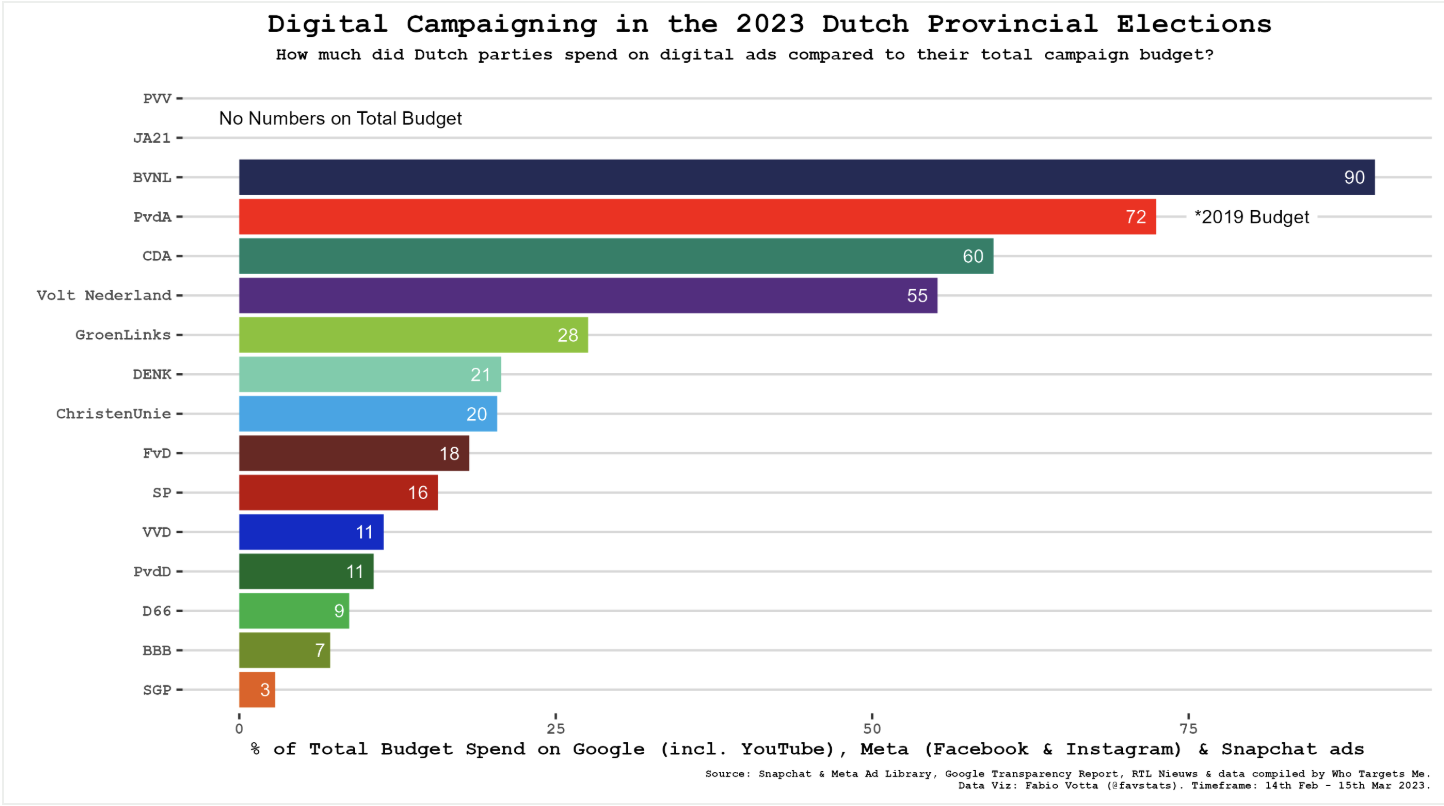
\includegraphics{pic/dutch_election.png}
\end{frame}

\begin{frame}{Research Questions}
\phantomsection\label{research-questions}
\begin{enumerate}
\tightlist
\item
  Do parties pay the same price for ads?
\end{enumerate}

\vspace{.5cm}
\pause

\begin{enumerate}
\setcounter{enumi}{1}
\tightlist
\item
  What drives price differences?
\end{enumerate}
\end{frame}

\begin{frame}{Why Is the Fairness of Online Competition Hard to Study?}
\phantomsection\label{why-is-the-fairness-of-online-competition-hard-to-study}
\begin{enumerate}
  \item Observational studies face many confounders:
    \begin{itemize}
      \item content, account history, agenda, targeting criteria
    \end{itemize}
  \vspace{.2cm}
  \pause

  \item Sock-puppet experiments:
    \begin{itemize}
      \item lack external validity
    \end{itemize}
  \vspace{.2cm}
  \pause

  \item Our approach: Audit study using real party accounts
\end{enumerate}
\end{frame}

\begin{frame}{Builds upon Votta et al.~2024}
\phantomsection\label{builds-upon-votta-et-al.-2024}
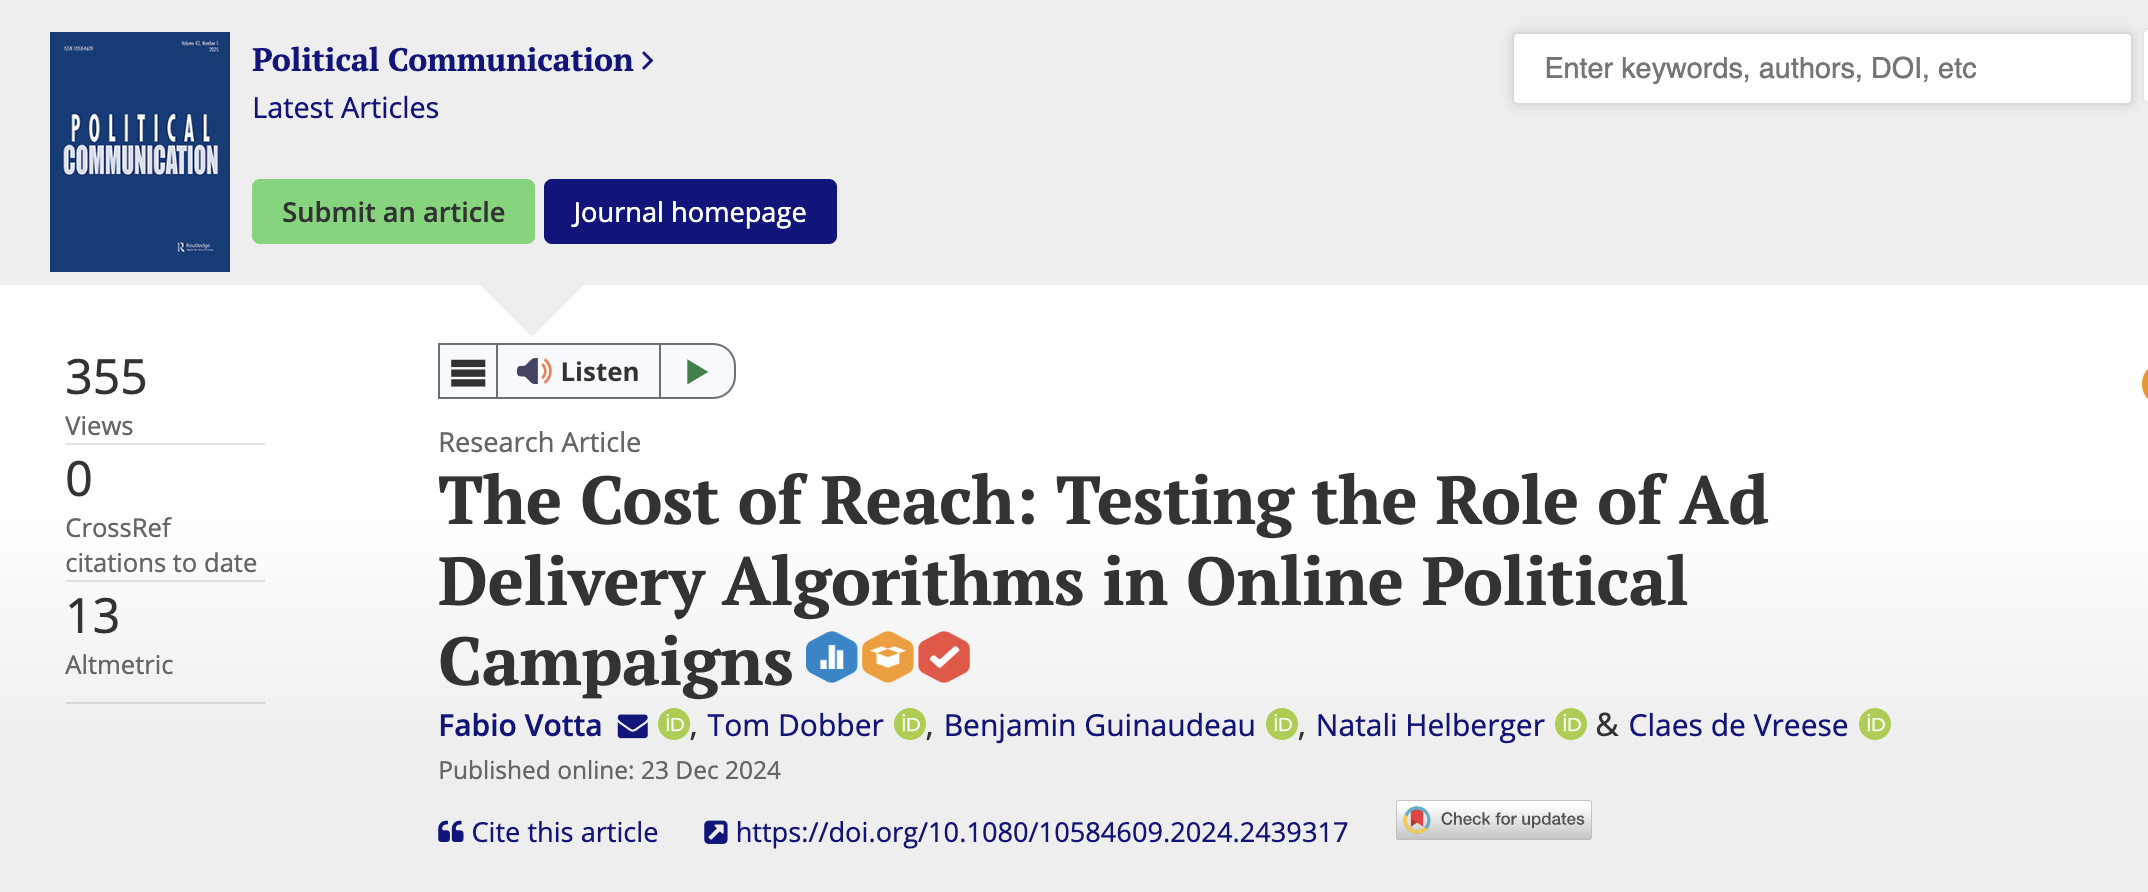
\includegraphics{pic/pol_com.png}
\end{frame}

\begin{frame}{Design}
\phantomsection\label{design}
\begin{enumerate}
  \item \textbf{Context:}
    \begin{itemize}
      \item 2024 European elections (June)
      \item Facebook and Instagram
    \end{itemize}
    \vspace{.2cm}
    \pause

  \item \textbf{Approach:}
    \begin{itemize}
      \item Real party accounts (30 parties across 8 countries)
      \item Identical "get-out-the-vote" ads with same targeting settings
      \item €1/day for 7 days (April 29, 2024 start)
      \item Outcome: Cost per 1,000 users reached
    \end{itemize}
    \vspace{.2cm}
    \pause

  \item \textbf{Targeting conditions:}
    \begin{itemize}
      \item No targeting
      \item Interested in politics (most-likely)
      \item Below-university education (least-likely)
    \end{itemize}
    \vspace{.2cm}
    \pause

  \item \textbf{Implications:}
    \begin{itemize}
      \item Equal prices would suggest that targeted ads do not distort competition
    \end{itemize}
\end{enumerate}
\end{frame}

\begin{frame}{Do Parties Pay the Same Price?}
\phantomsection\label{do-parties-pay-the-same-price}
\begin{itemize}
  \item \textbf{High variance across countries}
\end{itemize}

\begin{center}
    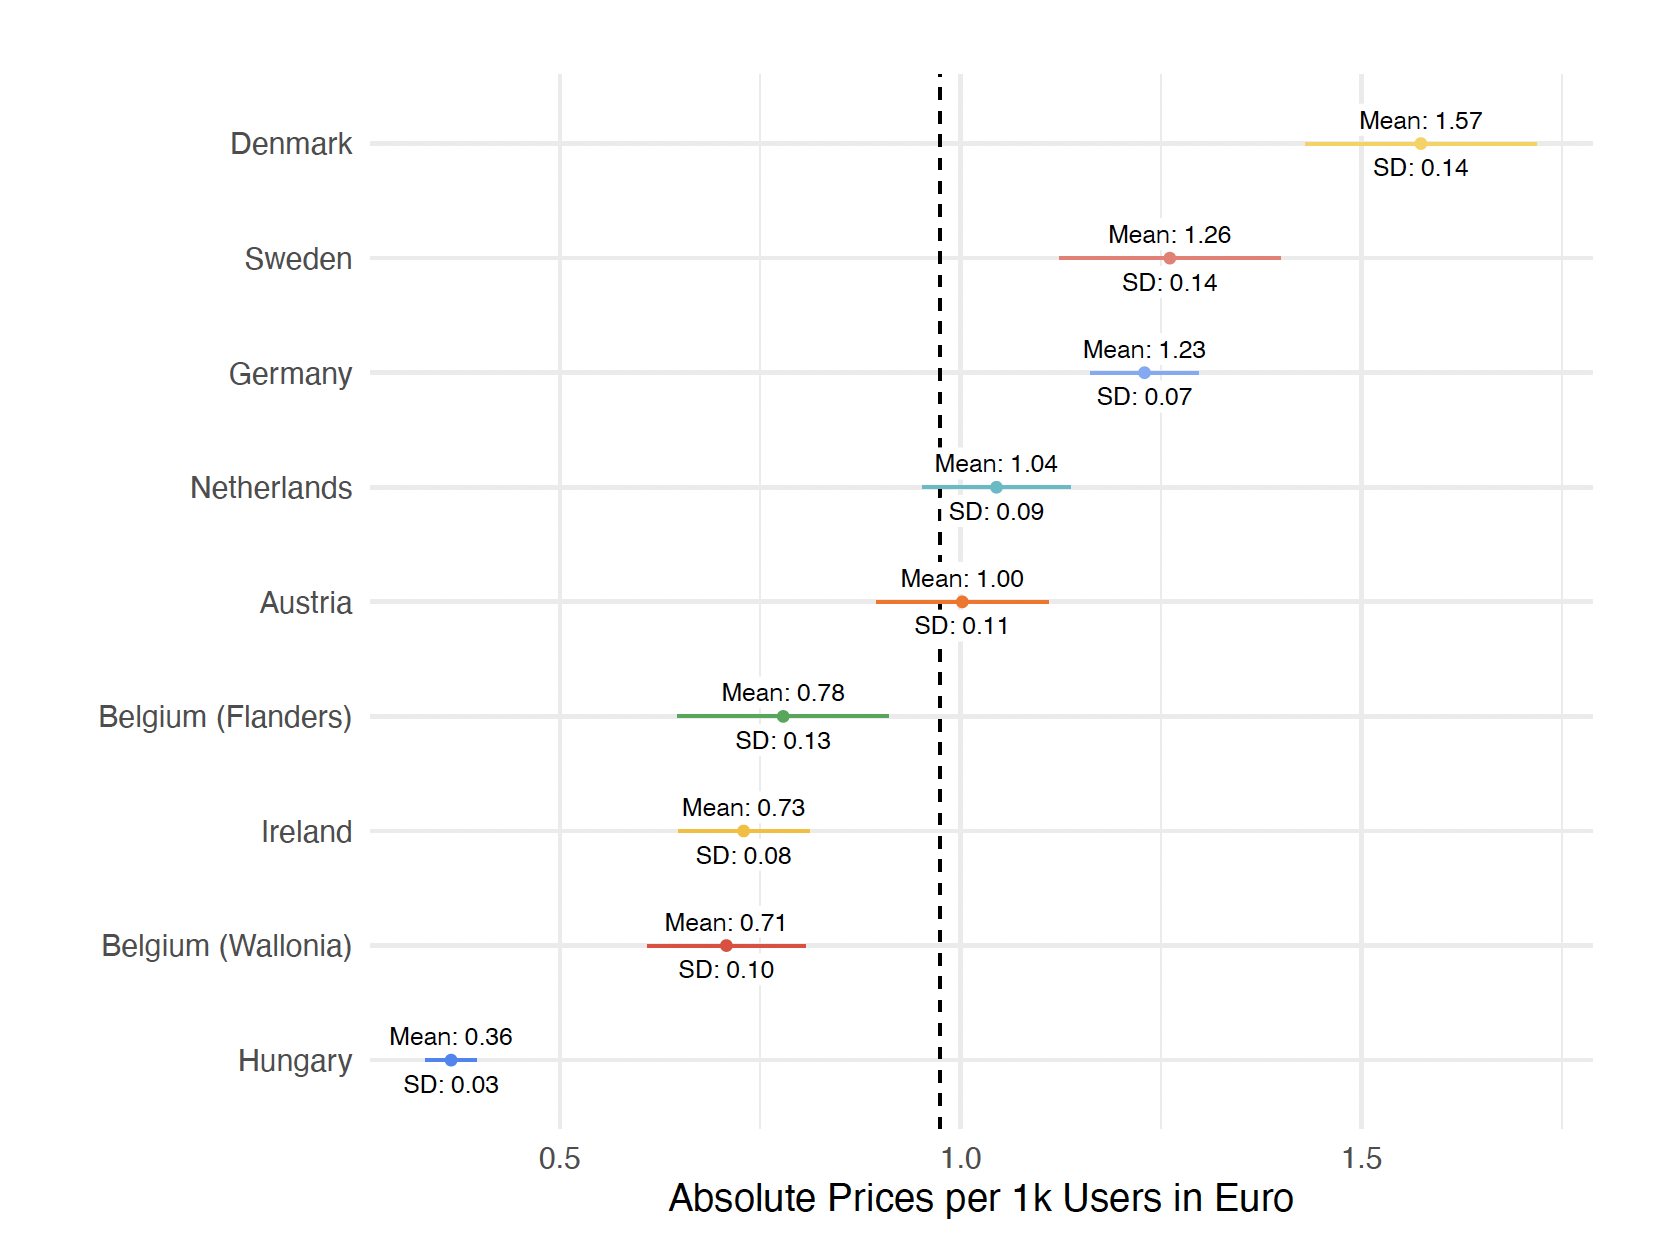
\includegraphics[height=\textheight]{pic/countries.png}
\end{center}
\end{frame}

\begin{frame}{Do Parties Pay the Same Price?}
\phantomsection\label{do-parties-pay-the-same-price-1}
\begin{itemize}
  \item \textbf{Within-country differences}:
\begin{itemize}
   \item 4\% average variation (max 27\%)
   \item Small differences but millions of additional campaign reaches
\end{itemize}
\end{itemize}

\begin{center}
    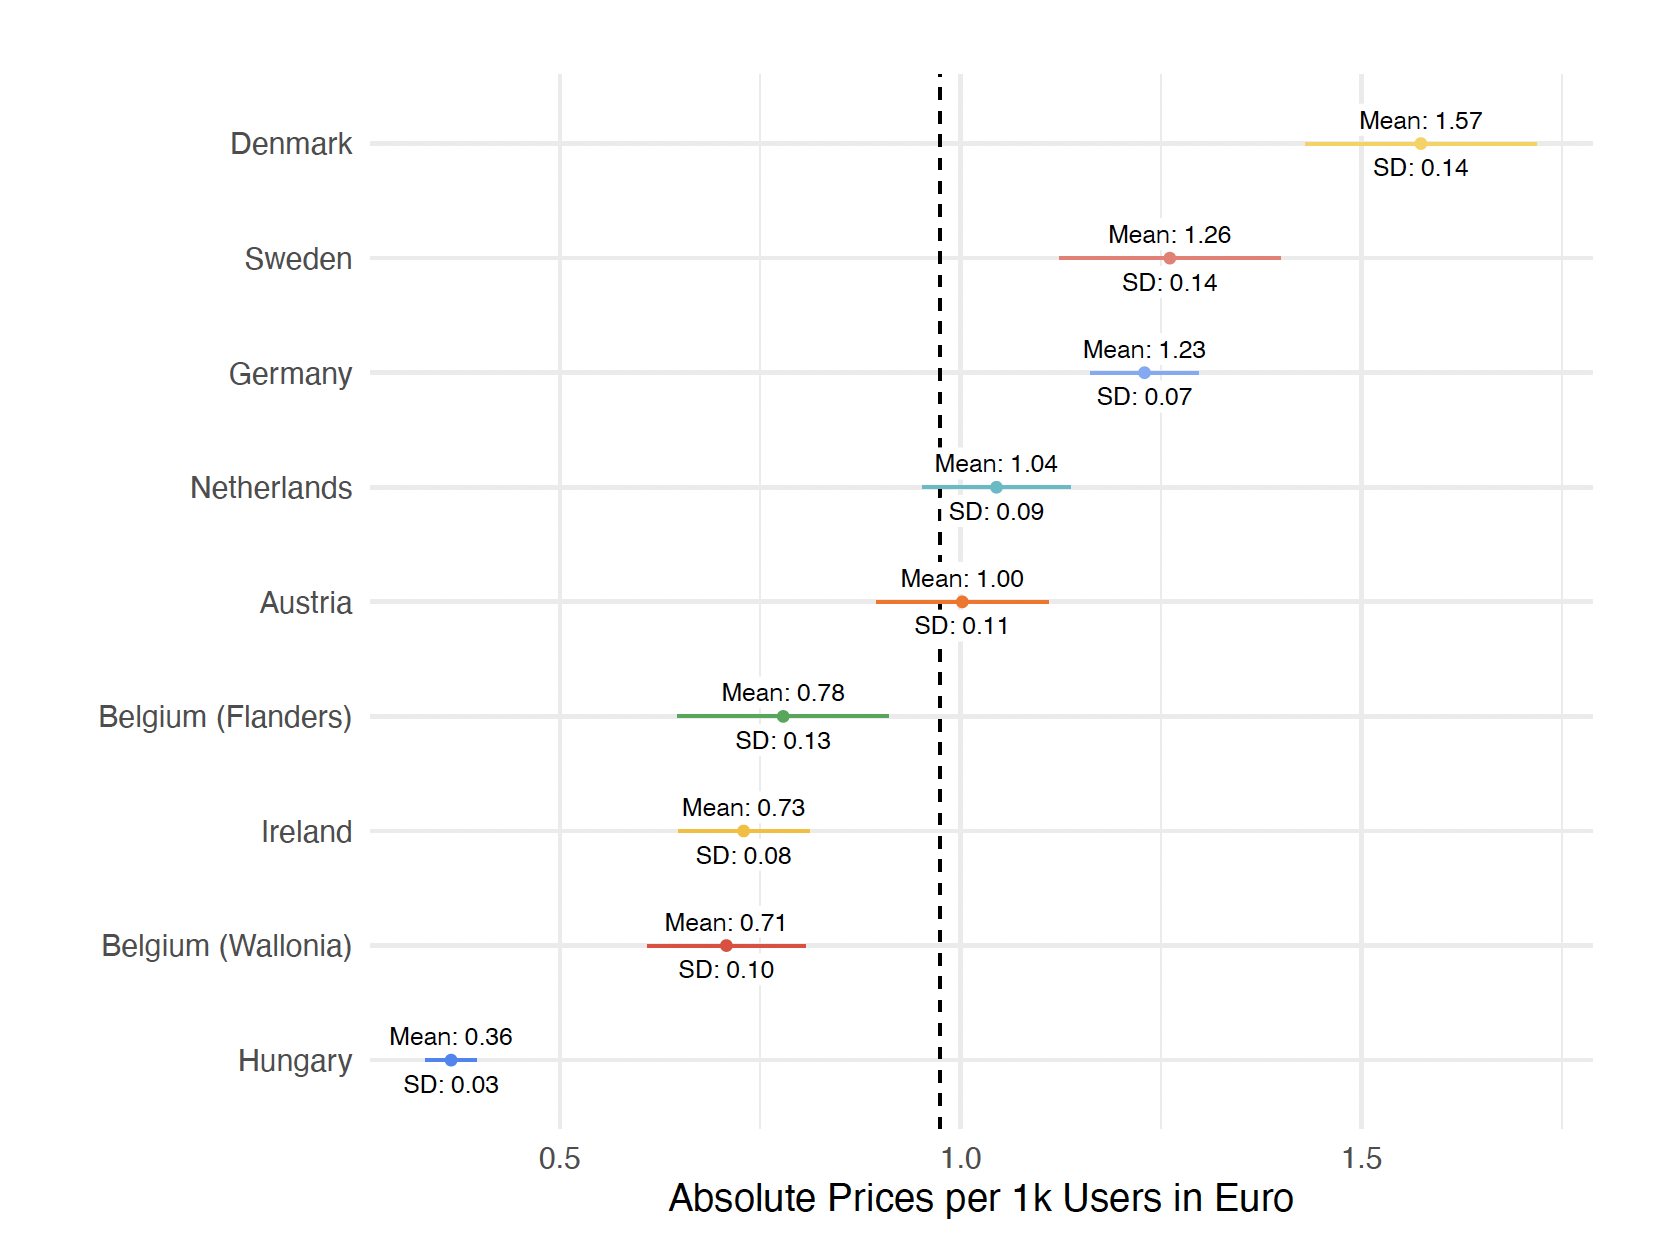
\includegraphics[height=0.8\textheight]{pic/countries.png}
\end{center}
\end{frame}

\begin{frame}{Do Parties Pay the Same Price?}
\phantomsection\label{do-parties-pay-the-same-price-2}
\begin{itemize}
\item \textbf{Most variation with "No Targetting"}
\begin{itemize}
  \item algorithm more free $\rightarrow$ more bias
\end{itemize}
\end{itemize}

\vspace{.5cm}

\begin{center}
    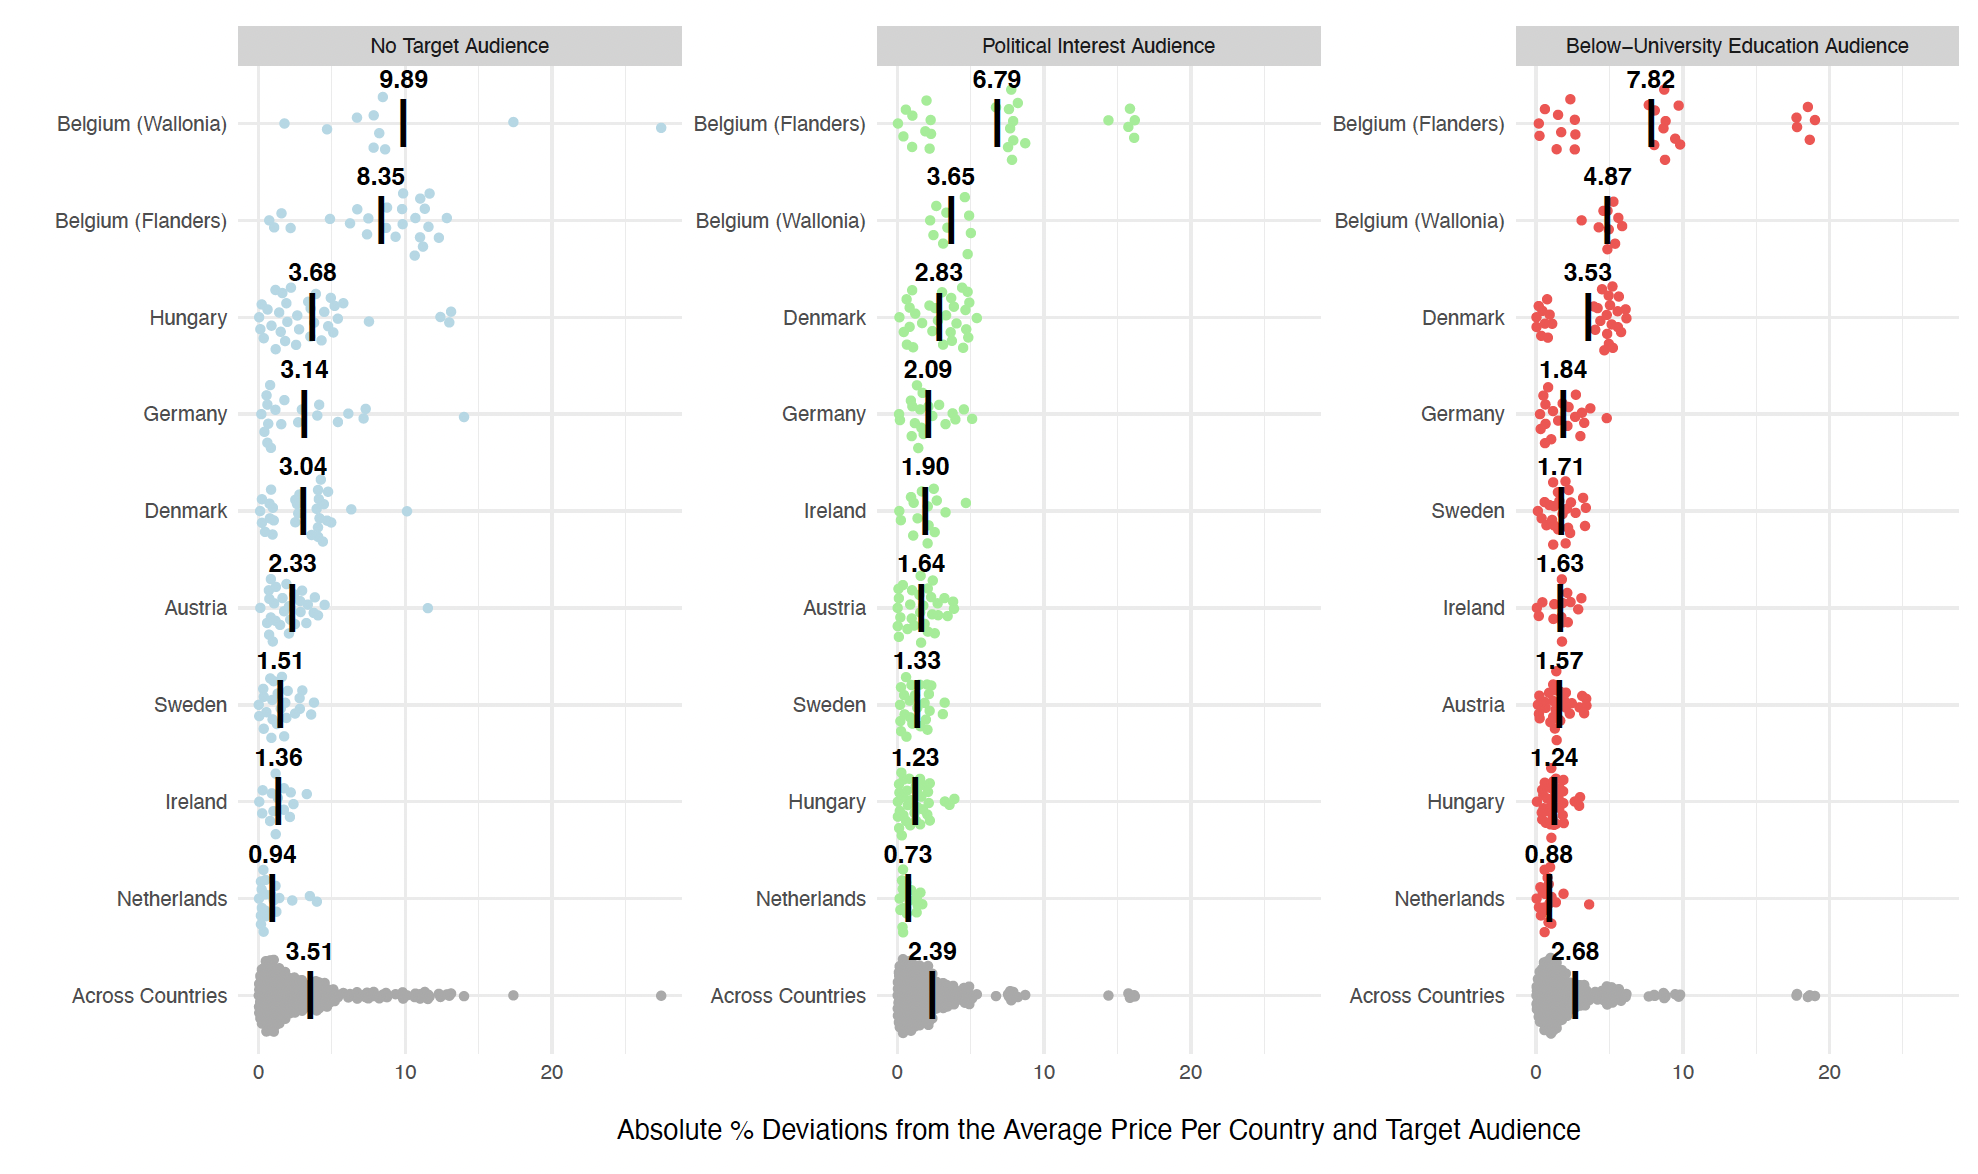
\includegraphics[height=0.8\textheight]{pic/conditions.png}
\end{center}
\end{frame}

\begin{frame}{Three Types of Factors Likely to Affect the Price
Differences}
\phantomsection\label{three-types-of-factors-likely-to-affect-the-price-differences}
\begin{enumerate}
\tightlist
\item
  \textbf{Account-level factors:}

  \begin{itemize}
  \tightlist
  \item
    Spending history, engagement patterns
  \end{itemize}
\end{enumerate}

\vspace{.2cm}
\pause

\begin{enumerate}
\setcounter{enumi}{1}
\tightlist
\item
  \textbf{Party-level factors}:

  \begin{itemize}
  \tightlist
  \item
    Ideology, electoral performance
  \end{itemize}
\end{enumerate}

\vspace{.2cm}
\pause

\begin{enumerate}
\setcounter{enumi}{2}
\tightlist
\item
  \textbf{Market-level factors}:

  \begin{itemize}
  \tightlist
  \item
    Audience size, ad competition
  \end{itemize}
\end{enumerate}
\end{frame}

\begin{frame}{What Drives Price Differences?}
\phantomsection\label{what-drives-price-differences}
\Large\textcolor{red}{%
  \faExclamationTriangle\; Disclaimer: Low statistical power requires caution when drawing conclusions \faExclamationTriangle\;
}
\end{frame}

\begin{frame}{What Drives Price Differences?}
\phantomsection\label{what-drives-price-differences-1}
\begin{center}
    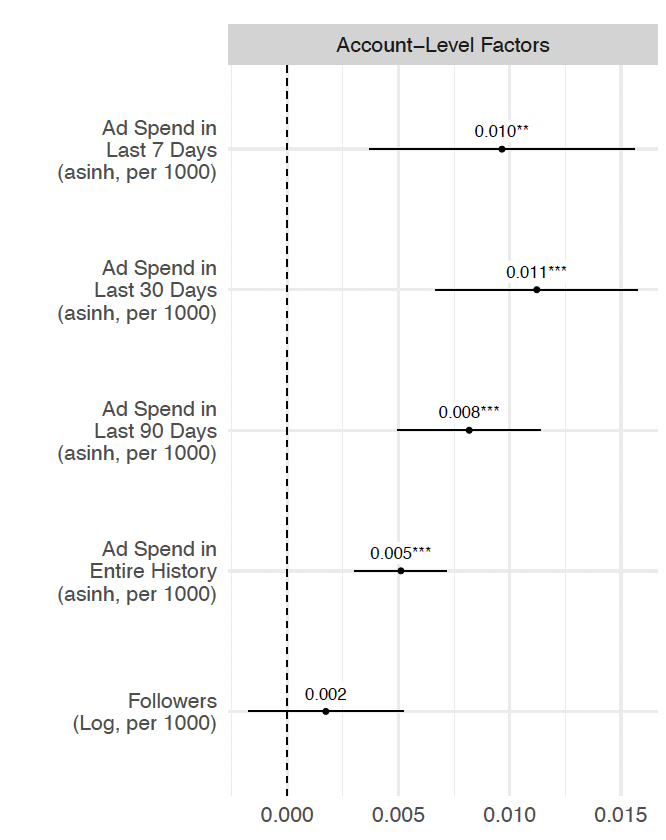
\includegraphics[height=\textheight]{pic/account.png}
\end{center}
\end{frame}

\begin{frame}{What Drives Price Differences?}
\phantomsection\label{what-drives-price-differences-2}
\begin{center}
    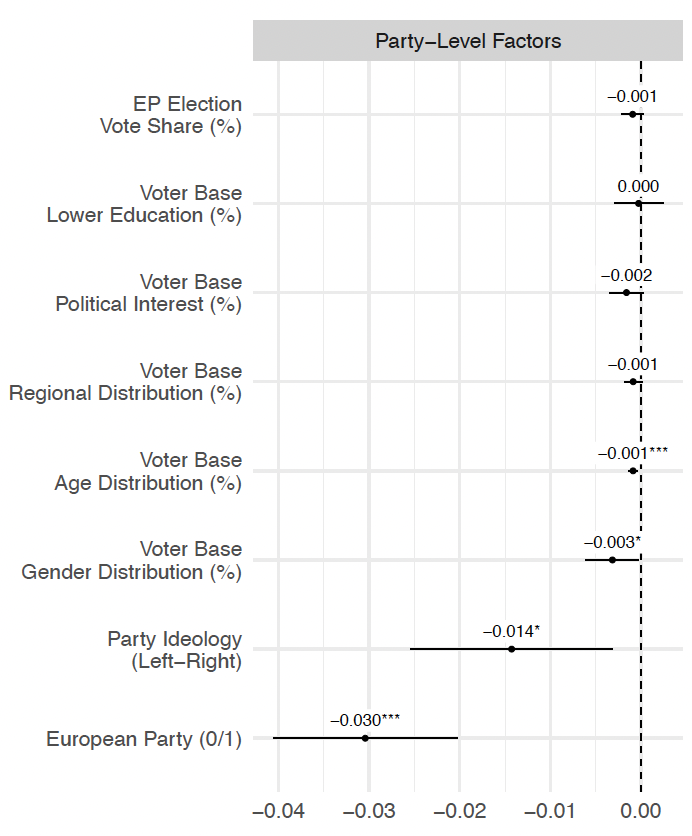
\includegraphics[height=\textheight]{pic/party.png}
\end{center}
\end{frame}

\begin{frame}{What Drives Price Differences?}
\phantomsection\label{what-drives-price-differences-3}
\begin{center}
    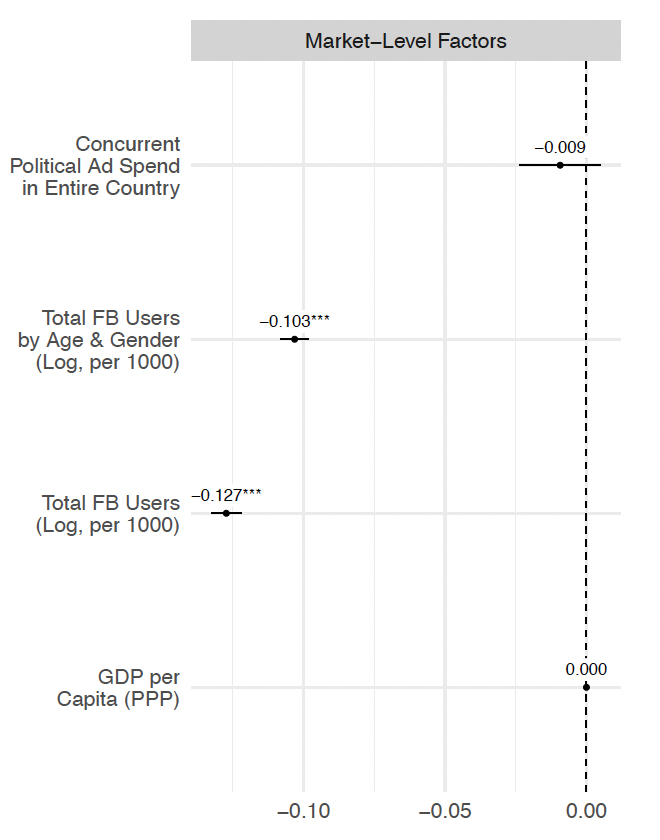
\includegraphics[height=\textheight]{pic/market.png}
\end{center}
\end{frame}

\begin{frame}{Conclusion}
\phantomsection\label{conclusion}
\begin{enumerate}
  \item Ad algorithms (unintentionally) favor some political actors
  \vspace{.2cm}
  \pause

  \item Within-country price variation:
    \begin{itemize}
      \item Average 4\% (max 27\%)
      \item Significant exposure bias
    \end{itemize}
  \vspace{.2cm}
  \pause

  \item Key drivers:
    \begin{itemize}
      \item Audience size
      \item Spending history
      \item Ideology (?)
      \item Transnational parties (?)
    \end{itemize}
  \vspace{.2cm}
  \pause

  \item Calls for stricter regulation to preserve democracy
    \begin{itemize}
      \item Algorithmic fairness
      \item Algorithmic access for independent researchers
    \end{itemize}
\end{enumerate}
\end{frame}

\end{document}
